%% LyX 2.1.1 created this file.  For more info, see http://www.lyx.org/.
%% Do not edit unless you really know what you are doing.
%%kp: \documentclass[english]{article}
%%kp: \usepackage[T1]{fontenc}
%%kp: \usepackage[latin9]{inputenc}
%%kp: \usepackage{babel}
%%kp: \usepackage{latexsym}
%%kp: \usepackage{amstext}
%%kp: \usepackage{graphicx}
%%kp: \usepackage[unicode=true]
%%kp:  {hyperref}

%%kp: \makeatletter
%%kp: \AtBeginDocument{
%%kp:   \def\labelitemiii{\(\rhd\)}
%%kp:   \def\labelitemiv{\(\oplus\)}
%%kp: }
%%kp: 
%%kp: \makeatother
%%kp: 
%%kp: \begin{document}

%%kp: \title{Tracking Corrections}
%\section{Tracking Corrections}
\subsection{Tracking Corrections}
%%kp: 
%%kp: \maketitle
%%kp: 
%%kp: \section{Introduction}

This work is mostly based on the work documented in the \href{https://www.jlab.org/Hall-B/secure/eg1-dvcs/technotes/targetinfo/target_info.pdf}%{EG1-DVCS technical note \#{} 4}
{EG1-DVCS-TN-004} %xz: you can be consistent and say this as you do below.
by P. Bosted \cite{trkCorNote}, in which a routine or method is developed
to swim the particles through the field map of the target magnet to
the drift chambers in order to determine the particle angles and position
at the target, provided the direction cosines of the tracks at DC
and the beam position from the raster magnets are known. It is expected
that the method improves both the angular resolution and the reconstructed
logitudinal vertex position. The slightly modified version of the
corresponding C/C++ routine is used with some of the constants in
the routine replaced by new parameters to be determined by the method
of \textbf{$\chi^{2}$-square minimization} using ep-elastic events.
%(We tried to find $e^{+}e^{-}$ pairs in our data set to use in the minimization just like in the EG1DVCS, but due to various reasons, we were unable to find them, and, therefore, had to settle with the ep-elastic events only).
(Since this data set didn't have enough $e^{+}e^{-}$ pairs, we didn't use them in the minimization like in the EG1DVCS.) %xz: "due to various reasons" What reasons?  SHould explain. If unknown, say unknown.


%\subsection{Method}
\subsubsection{Method}

First of all, in order to convert raster magnet ADCs into corresponding beam positions x0 and y0,
we need conversion parameters. These parameters are determined by using a method outlined in
\href{https://www.jlab.org/Hall-B/secure/eg1-dvcs/technotes/raster/raster.pdf}{EG1-DVCS-TN-002}.
The method determines the values of the slopes and offsets that convert the X- and Y-raster ADC readings to 
corresponding beam positions x0 and y0 in cm by minimizing the sensitivity of target vertex position (vz) 
for charged tracks to beam motion. 


Next, ep-elastic events are skimmed (from all of the \textbf{$NH_{3}$}
target data-set) using electron ID cuts for the electrons (see section \ref{allCuts}) in the sixth sector and proton ID consisting mainly of the time-of-flight cuts are used to select protons in the third sector (opposite to the sixth one). Then missing momentum cuts (less than 0.1 GeV for each of the four components Px, Py, Pz and E) based on 4-momentum conservation requirements (within measurement uncertainties) are used to help further clean up the accidental coincidences. These skimmed events are saved in root files and later reused for the minimization process described here.


The cuts used in the initial data skimming required that each of the four missing components be less than 0.1 GeV.

After that a correction routine involving a set of correction
equations with several unknown parameters are established. Then
with the help of TMinuit (ROOT version of Minuit), several sets of
trial values are given to these unknown parameters and the corresponding
correction is applied to the particles in the skimmed events. For
each set of these trial values, a specifically defined \textbf{$\chi^{2}$
}(see below) is evaluated looping over all the skimmed events and
the Minuit tries to find the optimum set of these parameter values
for which the \textbf{$\chi^{2}$} is minimum. Such an optimal
set of values are chosen as the correct values of these parameters
and is used in the eventual correction routine.


%\subsection{The correction routine}
\subsubsection{The correction routine}

The routine uses 17 constants (free parameters determined by the above mentioned process
of $\chi^{2}$-minimization) and the following input and output variables:
\begin{itemize}
\item \textbf{Input variables:} $x_{r}$, $y_{r}$, cxdc, cydc, xdc, ydc,
zdc, p, q. 

\begin{itemize}
\item $x_{r,}$, $y_{r}$ are x \& y beam positions as returned by the raster
correction routine (see appendix)
\item \textbf{cxdc, cydc} are direction cosines of the track as measured
at DC1
\item \textbf{xdc, ydc, zdc} are the coordinates of the track meausred at
DC1
\item p, q are the momentum and charge of the track
\end{itemize}
\item \textbf{Output variables:} cxc, cyc, czc, vzc (all three corrected
direction cosines and the corrected Z-coordinate at the vertex) .
\end{itemize}
The sequence of calculation steps taken (inside the routine) to arrive
at the output results are as follows (where, I am also using the notations
of P. Bosted i.e., subscripts '0' used to indicate variables at vertex,
subscript 'f' for those at the drift chambers (these are the tl1\_
variables in the ntuples), and the values of (x, y, z) are in cm):
\begin{itemize}
\item First of all, get ready the following constants and variables:

\begin{itemize}
\item \textbf{$f_{c}=\frac{B}{50}=0.995$} is the overall field correction 

\begin{itemize}
\item (i.e., the $B.dl$ correction factor. Our $B=4.97T$, with B in kG
$f_{c}$ is 0.995)
\end{itemize}
\item $targsign=1$
\item $\theta_{f}=acos(cz_{dc})$
\item $\phi_{f}=atan2(cy_{dc},cx_{dc})$
\end{itemize}
\item Then, $\theta_{f}$ is corrected (for the misalignment of the DC) as follows:

\begin{itemize}
\item If it's the electron in the event,

\begin{itemize}
\item $\theta_{f}=\theta_{f}+(\mathbf{par[0]}+\mathbf{par[1]}\times\phi_{f})\thinspace\frac{cos\theta_{f}}{cos\phi_{f}}+(\mathbf{par[2]}+\mathbf{par[3]}\times\phi_{f})\thinspace sin\theta_{f}$
\end{itemize}
\item else if its the proton, 

\begin{itemize}
\item $\theta_{f}=\theta_{f}+(\mathbf{par[4]}+\mathbf{par[5]}\times\phi_{f})$ \\

\end{itemize}
\end{itemize}
\item Next, get $\phi_{0}$ without raster corrections yet %(this accounts for the misalignment of the DC).

\begin{itemize}
\item $\phi_{0}=\phi_{f}+targsign\times f_{c}\thinspace(0.186+\mathbf{par[10]}+(0.045+\mathbf{par[11]})\thinspace\theta^{2}+(0.008+\mathbf{par[12]})\thinspace\theta_{f}^{3}+(0.0032+\mathbf{par[13]})\thinspace\theta_{f}^{3}/p^{2})\thinspace\frac{q}{p}$
\end{itemize}
\item Correction to polar angle from focusing effect. First, get focusing
term for beam (x,y)=0. 

\begin{itemize}
\item $\delta\theta=f_{c}\thinspace(0.90\thinspace\theta_{f}+1.2\thinspace\theta_{f}^{3})/(100\thinspace p^{2})$
\end{itemize}
\item Displacement of beam along trajectory ($x_{p}$) and perpendicular
to it ($y_{p}$) 

\begin{itemize}
\item $x_{p}=x_{r}\thinspace cos\phi_{0}+y_{r}\thinspace sin\phi_{0}$ 
\item $y_{p}=-(x_{r}+\mathbf{par[6]})\thinspace sin\phi_{0}+(y_{r}+\mathbf{par[7]})\thinspace cos\phi_{0}$ 
\end{itemize}
\item Correction to $\delta\theta$ from radial target field, which only
depends on raster x and y but not vertex z. Also, no effect on peak
at zero! 

\begin{itemize}
\item $\delta\theta=\delta\theta\thinspace(1.+targsign\thinspace q\thinspace p\thinspace(0.5/\theta_{f})\thinspace(y_{p}/0.75))$
\end{itemize}
\item Now can get cz 

\begin{itemize}
\item $\theta_{0}=\theta_{f}+\delta\theta$
\item $cz_{c}=cos\theta_{0}$
\end{itemize}
\item Now $\phi_{0}$ again, this time including raster correction 

\begin{itemize}
\item $\phi_{0}=\phi_{f}+targsign\thinspace f_{c}\thinspace(0.186+\mathbf{par[10]}+(0.045+\mathbf{par[11]})\thinspace\theta^{2}+(0.008+\mathbf{par[12]})\thinspace\theta_{f}^{3}+(0.0032+\mathbf{par[13]})\thinspace\theta_{f}^{3}/p^{2})\thinspace\frac{q}{p}\thinspace(1-(0.09+\mathbf{par[14]})\thinspace\frac{0.35-\mathbf{par[15]}}{\theta_{f}}\thinspace x_{p})$
\end{itemize}
\item Get cx and cy using this cz 

\begin{itemize}
\item $cx_{c}=sin\theta_{0}\thinspace cos\phi_{0}$
\item $cy_{c}=sin\theta_{0\thinspace}sin\phi_{0}$
\end{itemize}
\item Renomalize czc 

\begin{itemize}
\item $cz_{c}=\sqrt{1.0-cx{}_{c}^{2}-cy{}_{c}^{2}}$
\end{itemize}
\item \textbf{Apply target field rotation correction} 

\begin{itemize}
\item $cx_{c}=cx_{c}-targsign\thinspace q\thinspace\mathbf{par[8]}\thinspace cz_{c}/p$
\item $cy{}_{c}=cy_{c}+targsign\thinspace q\thinspace\mathbf{par[9]}\thinspace cz_{c}/p$
\end{itemize}
\item \textbf{Renormalize again:}

\begin{itemize}
\item $czc=\sqrt{1.0-cx{}_{c}^{2}-cy{}_{c}^{2}}$
\item $\theta_{0}=acos(cz_{c})$ 
\end{itemize}
\item \textbf{Get vertex z in cm} 

\begin{itemize}
\item $r_{dc}=\sqrt{(x_{dc}-x_{r})^{2}+(y_{dc}-y_{r})^{2}}$
\item $Z_{c}=Z_{dc}-\frac{r_{dc}-(22+\mathbf{par[16]})\thinspace cos\theta_{0\thinspace}(tan\theta_{0}-tan\theta_{f})}{tan\theta_{f}}$
\end{itemize}
\item Finally, the routine outputs (returns) the four corrected quantities

\begin{itemize}
\item \textbf{$cx_{c},cy_{c},cz_{c},Z_{c}$.}
\end{itemize}
\end{itemize}




%\subsection{Calculation of $\chi^{2}$ (to be minimized) }
\subsubsection{Calculation of $\chi^{2}$ (to be minimized) }

The chi-square has different components as follows:

$\mathbf{\chi^{2}=\chi_{Zvar}^{2}(e)+\chi_{Zvar}^{2}(p)+\chi_{Evar}^{2}+\chi_{miss}^{2}+\chi_{Ppen}^{2}+\chi_{Epen}^{2}+\chi_{Zpen}^{2}+\chi_{\Delta E}^{2}}$

where, 
\begin{itemize}
\item $\mathbf{\chi_{Zvar}^{2}(e)}$ and $\mathbf{\chi_{Zvar}^{2}(p)}$
are Z-variance contributions from electron and proton candidates in
the ep-elastic events and are calculated as $\mathbf{\chi}_{\mathbf{Zvar}}^{\mathbf{2}}=\frac{1}{N_{ep}-1}\Big(\sum Z_{c}^{2}-\frac{(\sum Z_{c})^{2}}{N_{ep}}\Big)/(0.05)^{2}$
separately for the electrons and protons. (Here, $Z_{c}$ is the corrected
$Z$ of vertex and $N_{ep}$ is the number ep-elastic events used
in the minimization)
\item $\mathbf{\chi}_{\mathbf{Evar}}^{\mathbf{2}}=\frac{1}{N_{ep}-1}\Big(\sum E_{b}^{2}-\frac{(\sum E_{b})^{2}}{N_{ep}}\Big)/(0.005)^{2}$
is $E_{b}$-variance contribution. (Here, $E_{b}=M_{p}\Big(\frac{1}{tan(\theta_{p})tan(\theta_{e}/2)}-1\Big)$
is the beam energy calculated after the angles are corrected by the
correction routine.)
\item $\mathbf{\chi}_{\mathbf{miss}}^{\mathbf{2}}=100\times\Big(\frac{\sum p_{x}^{2}(miss)+\sum p_{y}^{2}(miss)}{0.02^{2}}+\frac{\sum p_{z}^{2}(miss)+\sum E^{2}(miss)}{0.05^{2}}\Big)$
is missing four-momentum contribution. (Here, 100 is an arbitrary
number to make the weight of this contribution comparable to others.)
\item $\mathbf{\chi}_{\mathbf{Ppen}}^{\mathbf{2}}=\sum\limits _{i=0}^{16}\frac{(par[i]-iPar[i])^{2}}{0.01^{2}}$
is the contribution due to runawy penalty on free parameters of the
minimization. (Here, par{[}i{]} \& iPar{[}i{]} are the current and
initial values of the 'i'th parameter. In the first iteration, initial
values were set to either zeros or the corresponding values as determined
for EG1-DVCS by P. Bosted. In later iterations, they were set to the
values determined from the previous iteration of the minimization.)
\item $\mathbf{\chi}_{\mathbf{Zpen}}^{\mathbf{2}}=\sum\limits _{e,p}\Big(\sum\limits _{N_{ep}}\frac{(Z_{c}-(-100.93))^{2}}{0.05^{2}}\Big)$
is a penalty term when $Z_{c}$ runs away from the known/nominal target
center (-100.93 cm)
\item $\mathbf{\chi}_{\mathbf{Epen}}^{\mathbf{2}}=\sum\limits _{i=2}^{4}\Big(\frac{\sum\limits _{N_{ep}}E_{b}}{N_{ep}}-E_{0}\Big)^{2}/(0.005)^{2}$
is a pentalty term to constrain $E_{b}$ running away from the nominal
values $E_{0}$ of beam energy.
\item $\mathbf{\chi}_{\mathbf{\Delta E}}^{\mathbf{2}}=\Big(\sum\limits _{i=2}^{4}\frac{\sum\limits _{N_{ep}}(E_{b}-E_{0})^{2}}{N_{ep}}\Big)/(0.005)^{2}$
is another pentalty term to constrain $E_{b}$ running away from the
nominal values $E_{0}$ of beam energy.
\end{itemize}


%\subsection{Minimization }
\subsubsection{Minimization }

TMinuit is used to minimze the value of$\chi^{2}$ as calculated above
and, thereby, determine the values of the free parameters used in
the correction routine. The minimization was done in such a way that
the parameters were determined step by step - first deciding the first
six parameters (keeping others fixed to initial values), then next
two, then next two, then next four, then next 2 and finally the last
one respectively.


\subsubsection{Tracking Correction Results}

With the method of $\chi^{2}$-minimization described above, the following
set of values were determined for the 17 parameters from par{[}0{]}
through par{[}16{]} respectively:

-0.00165789, -0.00131314, -0.00643021, -0.00721441, -0.00775272, 0.00483673,
0.063387, -0.0615822, 0.00133127, 0.000839944, 0.0210091, -0.0363265,
0.00335536, 0.00104193, 2.51519, -0.0313527, -1.29325

As a result of the corrections with these newly determined parameter
values, various quantites before and after the corrections looked
as shown in the following figure:

%\begin{comment}
\begin{figure} [H]
%\includegraphics[scale=0.345]{Images/trkCorrPass2_ep}
\includegraphics[scale=0.345]{figuresEG4/FigKineCor/trkCorrPass2_ep}

\protect\caption{Comparing various quantities before and after the tracking corrections which affects only the angles (and not the magnitude 'p') of the momentum.}
\end{figure}








\begin{comment}
\subsection{Conclusion}

The new tracking correction routine for EG4 with our own values of
parameters (determined by the method of $\chi^{2}$-minimization using
ep-elastic events) gave just a little better result than the original
version of the routine that was developed by P. Bosted for EG1-DVCS
data.





\section{Appendix}


\subsection{Raster x \& y (in cm):}

Raster x and y (denoted as $x_{r}$ and $y_{r}$ in cms) come as output
from the \textbf{raster correction routine} that was developed during
the past EG4 (pass1) analysis. These are simply translations (into
centimeters) of raster ADC values as measured for the x and y arms
of the raster magnet system, and thus they represent the beam position
in the XY-plane located at the target position along the beam line.

The \textbf{raster correction routine} has 21 parameters deterimined
by a $\chi^{2}$- minimization process. 
\begin{verse}
Par{[}21{]} = \{3.42931e-05, 0.000422835, -4.07979e-05, -0.000420968,
4330.72, 4440.27, -101.022, 4129.42, 4340.07, -101.064, 4104.95, 4251.29,
-101.041, 4014.65, 3946.27, -101.052, 4192.43, 3343.59, -101.002,
0.00096982, 0.00201097\};
\end{verse}
It takes 9 variables as inputs:

$E_{i}$, q, $X_{ADC}$, $Y_{ADC}$, p, all three direction cosines
(cx, cy, cz) of the track and Z of the vertex.

(Here, Ei=0,1,2,3, \& 4 for 1.0, 1.3, 2.0, 2.3, \& 3.0 GeV data sets
respectively)
\begin{description}
\item [{And}] the routine returns four quantities: $x_{r}$, $y_{r}$,
corrected $\textrm{\ensuremath{\phi}}$ and corrected Z as outputs.
The calculations of the corrections are done as follows:\end{description}
\begin{itemize}
\item Calculate $\theta$ and $\phi$ at vertex using the direction cosines.
\item Calculate the sector angle ($\phi_{s}$) i.e. the $\phi$ of the sector
mid-plane (= $(Sector-1)\times60$.)
\item $Z_{cor}=Z+\frac{X_{p}}{tan(\theta)}+factor1\times factor2$ 
\item $\phi_{cor}=\phi-q\times50.0\times\frac{X_{p}}{100}\times\frac{1}{33.356\times P_{t}}$
where

\begin{itemize}
\item $X_{gain}=Par[0]+\frac{Par[1]}{E_{b}}$
\item $Y_{gain}=Par[2]+\frac{Par[3]}{E_{b}}$
\item $X_{offset}=Par[3\thinspace E{}_{i}+4]$
\item $Y_{offset}=Par[3\thinspace E{}_{i}+5]$
\item $x_{r}=(X_{ADC}-X_{offset})\thinspace X_{gain}$
\item $y_{r}=(Y_{ADC}-Y_{offset})\thinspace Y_{gain}$
\item $X_{p}=(x_{r}\thinspace cos\phi_{s}+y_{r}\thinspace sin\phi_{s})/cos(\phi-\phi_{s})$
\item $factor1=q\cdot10\cdot(Par[19]\cdot cx+Par[20]\cdot cy)\frac{1}{p\times sin\theta\times sin\theta}$; 
\item $factor2=\frac{1-0.25\times tan\theta\times tan\theta}{sin\theta\times cos\theta}$ 
\item $P_{t}=p\times sin\theta$
\end{itemize}
\end{itemize}
\begin{thebibliography}{1}
\bibitem[1]{key-1}Tracking from Drift Chambers to Target through
Solenoid (\href{https://www.jlab.org/Hall-B/secure/eg1-dvcs/technotes/targetinfo/target_info.pdf}{EG1-DVCS Techical Note \#{} 004}),
P. Bosted

\bibitem[2]{key-2} Raster Corrections, P. Bosted, S. Kuhn \& Y. Prok.
CLAS-NOTE-03-008.

\bibitem[3]{key-3}Momentum Corrections for E6, A. Klimenko \& S.
Kuhn. CLAS-NOTE-03-005.\end{thebibliography}

\end{document}

\end{comment}
